\documentclass[a4paper,notitlepage,10pt]{report}
\usepackage[left=2cm,right=2cm,top=2.5cm,bottom=2.5cm,footskip=1.25cm]{geometry}
\usepackage{enumitem,mathptmx,multicol,scrpage2,float}
\usepackage[dvipdfmx]{graphicx}
\usepackage{bmpsize,capt-of,microtype,subcaption,amsmath} %,siunitx
%\usepackage[none]{hyphenat}
\usepackage[belowskip=0pt,aboveskip=0pt]{caption}
\usepackage[hyphens]{url}
%\usepackage{natbib}
\ifoot[]{}
\cfoot[]{}
\ofoot[\pagemark]{\pagemark}
\pagestyle{scrplain}
\pagenumbering{arabic}
\DeclareGraphicsExtensions{.png,.jpg}
\newcommand{\tab}{\hspace{0.75cm}}
\newcommand{\fontTitle}{\fontsize{28pt}{30.8pt}\selectfont}
\newcommand{\fontHeading}{\fontsize{12pt}{13.2pt}\selectfont}
\newcommand{\fontSubHeading}{\fontsize{10pt}{11pt}\selectfont}
\newcommand{\fontName}{\fontsize{11pt}{12.1pt}\selectfont}
\newcommand{\fontBody}{\fontsize{10pt}{11pt}\selectfont}
\newcommand{\fontRef}{\fontsize{9pt}{9.9pt}\selectfont}
\newcommand{\sepTable}{\setlength{\intextsep}{12pt}}
\newcommand{\sepFigure}{\setlength{\intextsep}{10pt}}
\newenvironment{nscenter}
	{\parskip=0pt\par\centering}
	{\par\noindent\ignorespacesafterend}

\newcounter{sections}
\newcounter{subsections}[sections]
\newcounter{appendix}
\renewcommand{\theappendix}{\Alph{appendix}}

\sepFigure
\linespread{1.05}
\righthyphenmin=62
\abovedisplayskip=0pt\belowdisplayskip=0pt
\captionsetup[figure]{belowskip=0pt,aboveskip=5pt}
\captionsetup[table]{belowskip=0pt,aboveskip=6pt}
\renewcommand\UrlFont{\rmfamily}
%\bibliographystyle{plain}

\begin{document}
\parindent=0pt\parskip=0pt
\begin{center}
\fontTitle
D4 Design Project SPECIES Report
\vspace{25pt}

\fontName
Yubo Zhi

\fontBody
\textit{yz39g13@soton.ac.uk}

\fontBody
\textit{Personal Tutor: Professor Alun S Vaughan}
\vspace{25pt}

\end{center}

\fontBody
\begin{enumerate}[label={Abstract:},align=left,leftmargin=2cm,labelwidth=!,topsep=0pt,partopsep=0pt,parsep=0pt,itemsep=0pt]
\item
The objective of this project was to design a secure and mobile communication system in limited time and resources. The design was done by group of 6 students working as a team in 12 days, competing with 10 other teams. The system must be able to transmit human voice securely over short range wireless transmission, but could have any kinds of extensions as well. The prototype our team built utilities 2 Il Mattos, using high speed UART to communicate. The first one was for control and user friendly GUI with touchscreen, the second one was for wireless data communication, audio input and output. The device was able to transmit and receive human voice from microphone to speaker at the opponent end like a walkie talkie, simultaneous and shared sketching, send and receive text messages.
\end{enumerate}
\vspace{25pt}

\columnsep=0.7cm
\begin{multicols}{2}

% Contribution
\fontHeading
\stepcounter{sections}
\textbf{\thesections.\tab Contribution}
\vspace{10pt}

\fontBody
Favour in programming and familiar with C/C++ programming with the AVR and TFT display, I decided to do the programming part of Il Matto 1 including UART communication protocol between Il Matto 1 and Il Matto 2 to control audio transmission, and transmit varies type of data. The programming part include resistive touchscreen interface and GUI design, which were totally optional from the compulsory audio transmission of the project, but could add great features to our device. Diwen Hu (dh1g14) was helping me at overall GUI design, but not on the code side since he do not know much about C/C++ programming.
\vspace{6pt}

At the end of project, what I achieved were:
\vspace{6pt}

\begin{enumerate}[label={\arabic*)},align=left,leftmargin=0.5cm,labelwidth=!,topsep=0pt,partopsep=0pt,parsep=0pt,itemsep=0pt]
\item Menu selection GUI with multi-level submenus and scroll ability.
\item Resistive touchscreen working, and able to scroll and activate the menu items.
\item Resistive touchscreen sketch on TFT with full scale colour selection and 9 different brush sizes.
\item Lower case letter and punctuation text input through swiping on virtual keypad.
\item Easy and successful integration with Il Matto 2 through doubly buffered UART protocol with acknowledge.
\item Touch button controls Il Matto 2 audio transmission.
\item Ability to instantly transmit sketch to either side by half duplex.
\item Ability to send text messages and queued at the other side to ensure no messages loss.
\end{enumerate}
\vspace{10pt}

% Specification
\fontHeading
\stepcounter{sections}
\textbf{\thesections.\tab Specification}
\vspace{10pt}

\fontBody
The part I were responsible for is the direct interface with user, therefore an easy to use interface would be essential, so TFT display with resistive touchscreen for GUI interface was determined. A user authorisation method would be on the GUI side as well.
\vspace{6pt}

The UART protocol used to transfer data packages between Il Matto 1 and Il Matto 2 was using a baud rate of 750kbps, which was quite high. Therefore in order to ensure no data package could got lost, a communication protocol using interrupts and double buffer with acknowledge from opponent side was required.
\vspace{10pt}

% Design & Simulation
\fontHeading
\stepcounter{sections}
\textbf{\thesections.\tab Design \& Simulation}
\vspace{10pt}

% GUI design
\fontSubHeading
\stepcounter{subsections}
\textbf{\thesections.\thesubsections\tab GUI design}
\vspace{6pt}

\fontBody
The microcontroller used is 8bit AVR core ATmega644P, with Il Matto board. The TFT display is using ili9341 controller with a resolution of 320x240, connected to the Il Matto board through 8bit parallel interface with control pins at PORTA, data port at PORTC.
\vspace{6pt}

By looking at datasheet \ref{ref:ili9341} section 9.2.2 Vertical Scroll Mode, a menu selection with scroll ability were decided to be designed as primary GUI entry.
\vspace{6pt}

The vertical scroll mode shown by Figure \ref{fig:tftVS} was the base of fast scroll display of menu items.
\vspace{6pt}

\begin{figure}[H]
	\centering
	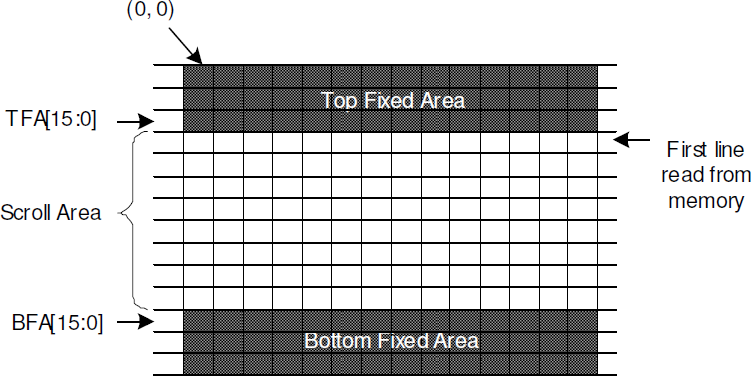
\includegraphics[width=0.9\columnwidth]{tft_vs}
	\caption{TFT Vertical scroll mode specification (adapted from \ref{ref:ili9341})}
	\label{fig:tftVS}
\end{figure}
\vspace{6pt}

Since the scroll mode in built into the TFT controller, by sending a 3 bytes command it was very easy to scroll the screen area. But there were some limitations, the scroll mode only apply to vertical orientation, and do not translate the coordinate from select area command, it only changes the line read from frame memory when the controller refreshing the TFT. Thus coordinate translation must be implemented from the programming side (implemented in tft.cpp from libtft-cpp \ref{ref:libtft-cpp}).
\vspace{6pt}

The difficulties were, functions for drawing rectangle and characters must be modified in order to mask out displays above the top fixed area and below the bottom fixed area, also continue drawing at the original bottom edge coordinate, which now may become the middle of display, and need to continue drawing from the original top edge coordinate, as illustrated by Figure \ref{fig:tftVSExample}.
\vspace{6pt}

\begin{figure}[H]
	\centering
	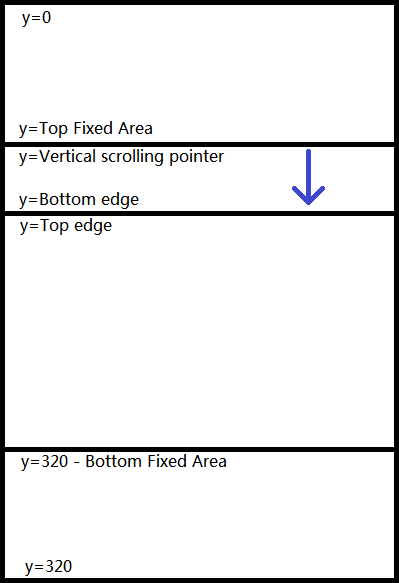
\includegraphics[width=0.6\columnwidth]{tft_vsexample}
	\caption{Example vertical scroll mode coordinates}
	\label{fig:tftVSExample}
\end{figure}
\vspace{6pt}

Originally landscape TFT orientation was decided, the menu item selection GUI designed as shown by photo \ref{fig:photoTSLandscape}.
\vspace{6pt}

\begin{figure}[H]
	\centering
	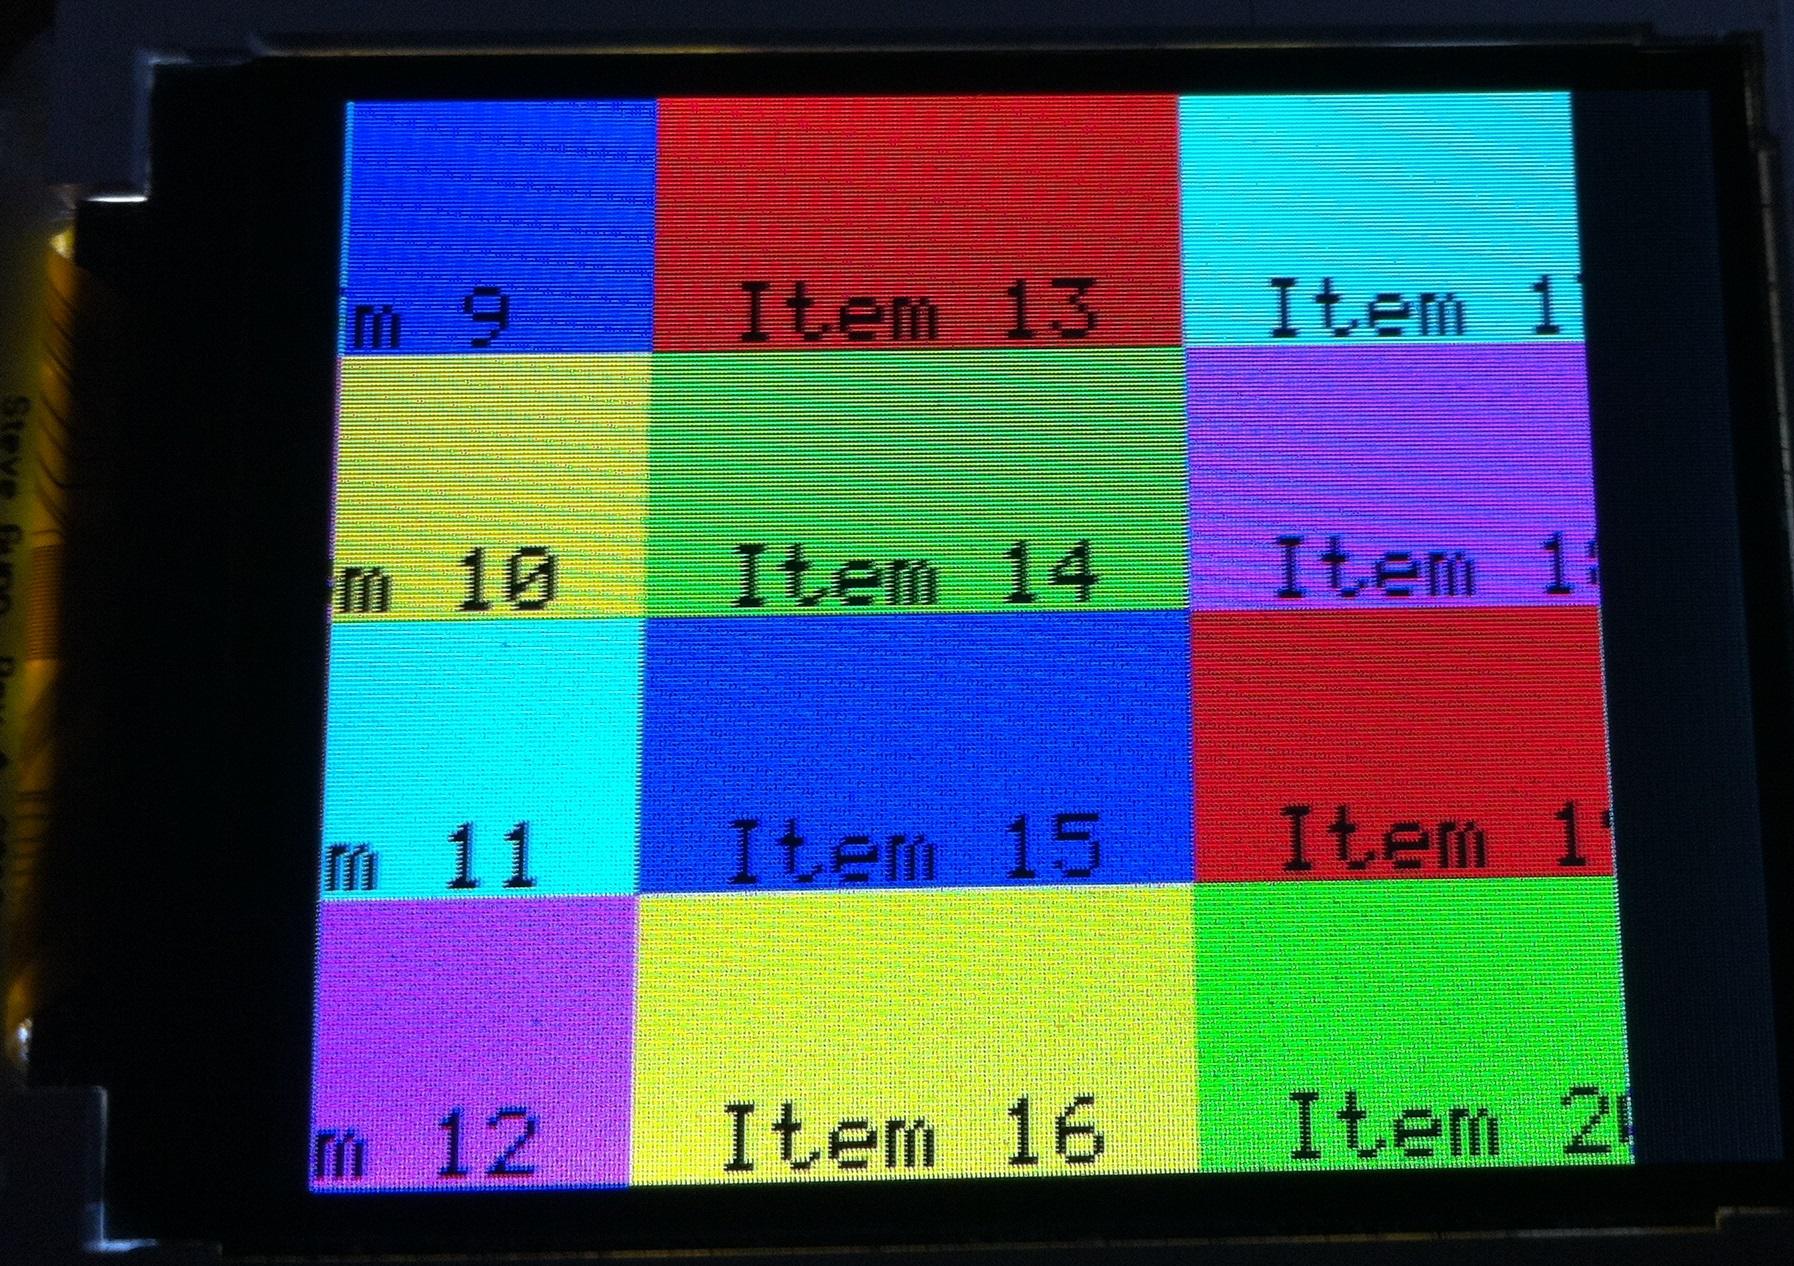
\includegraphics[width=0.9\columnwidth]{photo_ts_landscape}
	\caption{Menu selection GUI at landscape orientation}
	\label{fig:photoTSLandscape}
\end{figure}
\vspace{6pt}

But by constrains of touchscreen, the orientation later changed to portrait, which actually gave a better looking, also the coding of the menu selection became easier. Figure \ref{fig:capTFTPortrait} shows screen capture of the final product root menu at portrait. The final code was packed as liblist and available at \ref{ref:liblist}.
\vspace{6pt}

\begin{figure}[H]
	\centering
	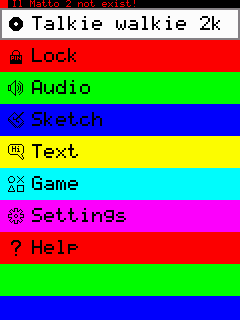
\includegraphics[width=0.5\columnwidth]{cap_tft_portrait}
	\caption{Menu selection GUI at portrait orientation}
	\label{fig:capTFTPortrait}
\end{figure}
\vspace{6pt}

% Resistive touchscreen design
\fontSubHeading
\stepcounter{subsections}
\textbf{\thesections.\thesubsections\tab Resistive touchscreen design}
\vspace{6pt}

\fontBody
The touchscreen used in our device is a 4-wire resistive touchscreen, it has 2 thin film with resistive coating, when pressure is applied to the touchscreen, the two layer contacts as demostrated in Figure \ref{fig:tsSide}.
\vspace{6pt}

\begin{figure}[H]
	\centering
	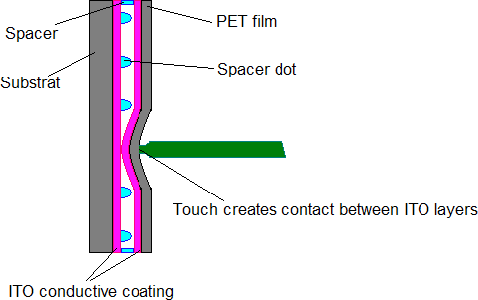
\includegraphics[width=0.8\columnwidth]{ts_side}
	\caption{Resistive touchscreens (adapted from \ref{ref:tsATMEL})}
	\label{fig:tsSide}
\end{figure}
\vspace{6pt}

The touchscreen can be modelled as shown by Figure \ref{fig:tsSCH}, when pressure applied the resistor $R_{Touch}$ would connect the top and bottom resistive layer.
\vspace{6pt}

\begin{figure}[H]
	\centering
	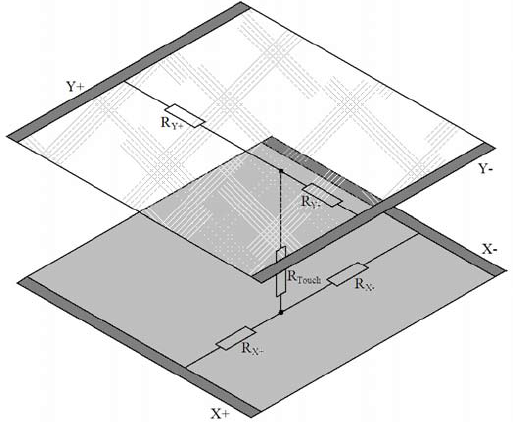
\includegraphics[width=0.8\columnwidth]{ts_sch}
	\caption{"Schematic" of a 4-wire touch screen when pressure is applied (adapted from \ref{ref:tsATMEL})}
	\label{fig:tsSCH}
\end{figure}
\vspace{6pt}

When detecting touchscreen press, connect Y layer to $V_{SS}$, attach a pull-up resistor at X+, than read the digital value of X+. If the touchscreen is pressed, X and Y layer connected, thus X+ would be pulled to $V_{SS}$.
\vspace{6pt}

When reading X value, apply $V_{CC}$ and $V_{SS}$ across X+ and X- terminals, put Y- terminal in high-Z mode, than read the voltage on Y+ terminal using ADC. The resistance of Y layer and $R_{Touch}$ could be ignored due to input impedance of ADC was very high ($100M\Omega$ on ATmega644P). By assuming the X layer was linear about resistance and x-coordinate, the X value therefore was the value output from the potential divider formed by $R_{X+}$ and $R_{X-}$, which was the voltage read from ADC directly.
\vspace{6pt}

Y value could be read by using the same method, apply $V_{CC}$ and $V_{SS}$ across Y+ and Y- terminals than read the voltage divided by $R_{Y+}$ and $R_{Y-}$.
\vspace{6pt}

In summary, by use the methods described in Table \ref{tb:ts}, the microcontroller could interfacing with the touchscreen with 2 ADC channels.
\vspace{6pt}

\sepTable
\begin{table}[H]
\caption{Touchscreen interfacing (adapted from \ref{ref:tsNXP})}
\label{tb:ts}
\begin{tabular}{p{0.15\columnwidth} p{0.2\columnwidth} p{0.1\columnwidth} p{0.1\columnwidth} p{0.1\columnwidth}}
	\hline
	Function	& X+	& Y+	& X-	& Y- \\ \hline
	Detection	& Digital input with pull-up	& Open	& Open	& $V_{SS}$ \\ \hline
	Read X	& $V_{CC}$	& ADC1	& $V_{SS}$	& Open \\ \hline
	Read Y	& ADC2	& $V_{CC}$	& Open	& $V_{SS}$ \\ \hline
\end{tabular}
\end{table}
\sepFigure

After read ADC data from touchscreen, it was necessary to map the data to the coordinate system of the display. The method of calibration can be found at \ref{ref:tsTI}, it was actually an image move and scale algorithm described using matrices. But bother to implement all the matrix operations, the calibration code was directly copied from an open source touchscreen library\ref{ref:tslib}.
\vspace{6pt}

The resistive 4-wire touchscreens ordered were 4.36in, which were even larger than two TFT displays with a size of 2.2in, the extra spaces could be used for other purposes.
\vspace{6pt}

Originally landscape orientation was chosen, the extra area of touchscreen would be used for permanent buttons, as illustrated by Figure \ref{fig:tsLandscape}.
\vspace{6pt}

\begin{figure}[H]
	\centering
	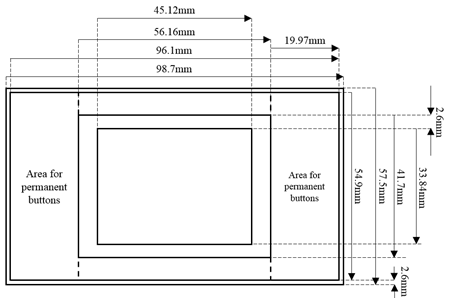
\includegraphics[width=0.75\columnwidth]{ts_landscape}
	\caption{Original landscape orientation layout (produced by ner1g13)}
	\label{fig:tsLandscape}
\end{figure}
\vspace{6pt}

However, the final orientation of the device decided to be portrait, with this arraignment, TFT display was places at the right part with portrait orientation of the touchscreen, while the left part of the touchscreen was used for virtual keypad with 4x4 buttons or colour and brush selection at sketch mode, as demonstrated in Figure \ref{fig:tsLayout}. Moreover, the device in portrait orientation results in a better look, and also made coding for TFT scrolling mode a lot easier.
\vspace{6pt}

\begin{figure}[H]
	\centering
	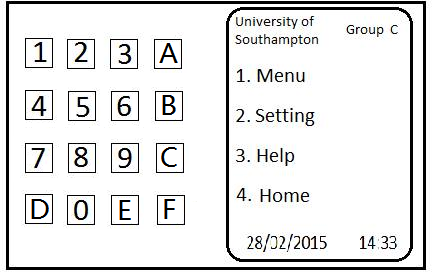
\includegraphics[width=0.6\columnwidth]{ts_layout}
	\caption{Portrait touchscreen layout (produced by dh1g14)}
	\label{fig:tsLayout}
\end{figure}
\vspace{6pt}

The calibration data were stored in the EEPROM built inside ATmega644P once calibration completed. Thus calibration process would not needed every time start up. If calibration failed, another mechanism also implemented. Recalibration will occurred when user power up the device while pressing the touchscreen, so that a re-flash of EEPROM was no longer needed.
\vspace{6pt}

% Sketch mode design
\fontSubHeading
\stepcounter{subsections}
\textbf{\thesections.\thesubsections\tab Sketch design}
\vspace{6pt}

\fontBody
The sketch mode draw rectangles on TFT centered at touched point. The numbers 1-9 on the virtual keypad were used to select brush sizes, which were actually the size of rectangles drawn. Full scale brush colour selection was done by swipe at the virtual keypad region as shown by Figure \ref{fig:keypad}. A second indicator located at top left indicates current brush size and colour. Figure \ref{fig:capSKT} demostrated the sketch mode. Source code for sketch mode were at software listing 10 and 11 with group report.
\vspace{6pt}

\begin{figure}[H]
	\centering
	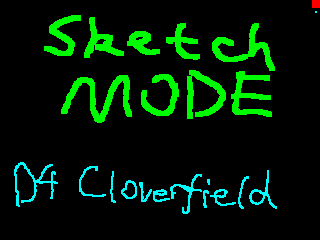
\includegraphics[width=0.6\columnwidth]{cap_skt}
	\caption{Screen capture of sketch mode}
	\label{fig:capSKT}
\end{figure}
\vspace{6pt}

\begin{figure}[H]
	\centering
	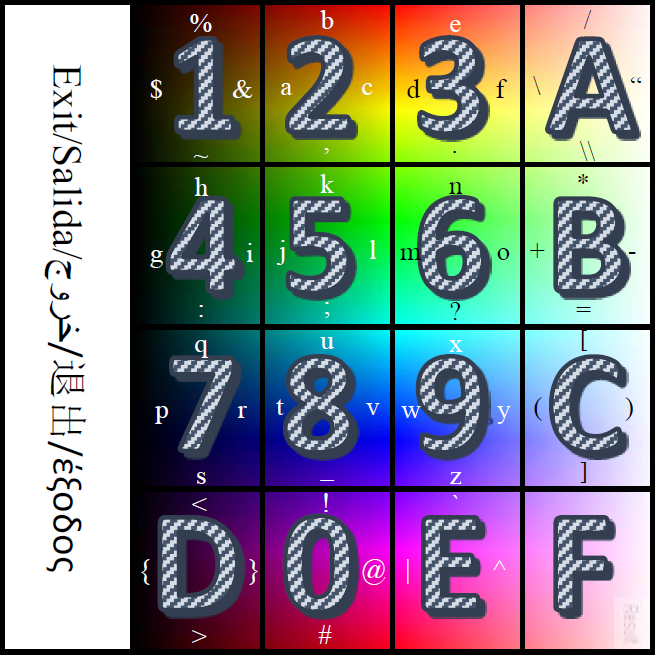
\includegraphics[width=0.6\columnwidth]{keypad}
	\caption{keypad drawings (produced by ner1g13)}
	\label{fig:keypad}
\end{figure}
\vspace{6pt}

In shared sketching mode, the sketch data was buffered and arranged into variable length packages then send to the other end wirelessly through Il Matto 2. The package structure will be described later in UART protocol section, the package data for shared sketching mode was arranged as following:

\begin{enumerate}[label={\arabic*)},align=left,leftmargin=0.5cm,labelwidth=!,topsep=0pt,partopsep=0pt,parsep=0pt,itemsep=0pt]
\item Type (1 byte), which is PKG\_TYPE\_SKETCH.
\item Size (1 byte), the brush size.
\item Colour (2 bytes), colour used throughout this package.
\item Coordinates (4 bytes array), unsigned 2 bytes x-coordinate followed by unsigned 2 bytes y-coordinate.
\end{enumerate}
\vspace{6pt}

% Pin authorisation design
\fontSubHeading
\stepcounter{subsections}
\textbf{\thesections.\thesubsections\tab Pin authorisation design}
\vspace{6pt}

The authorisation method designed was a typical 4 digits PIN passcode, input from the virtual keypad. A new passcode will be asked at first time EEPROM initialisation, and stored inside EEPROM, so would not lost after power down. The PIN can be later reseted at settings menu, but the original passcode will be required, a menu item also added to lock the device. No timeout or retry limits implemented currently. Data package were also handled while PIN locking, but notifications were not shown until device unlocked. Figure \ref{fig:capPINLocked} demonstrated the locked state.
\vspace{6pt}

\begin{figure}[H]
	\centering
	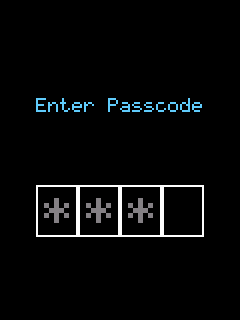
\includegraphics[width=0.4\columnwidth]{cap_pin_locked}
	\caption{PIN locked state screen capture}
	\label{fig:capPINLocked}
\end{figure}
\vspace{6pt}

% Text input design
\fontSubHeading
\stepcounter{subsections}
\textbf{\thesections.\thesubsections\tab Text input design}
\vspace{6pt}

The left extra area of touchscreen was used as virtual keypad, by attaching a piece of paper with a keypad printed on it, and a simple calibration procedure shown in Figure \ref{fig:capKPCAL}.
\vspace{6pt}

\begin{figure}[H]
	\centering
	\begin{subfigure}[b]{0.4\columnwidth}
		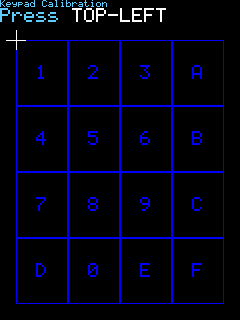
\includegraphics[width=\textwidth]{cap_kp_cal}
		\caption{Keypad calibration}
		\label{fig:capKPCAL}
	\end{subfigure}
	\begin{subfigure}[b]{0.4\columnwidth}
		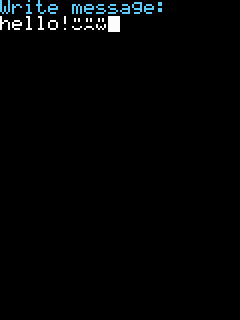
\includegraphics[width=\textwidth]{cap_text}
		\caption{Message writing}
		\label{fig:capText}
	\end{subfigure}
	\caption{Text input GUI}
	\label{fig:capTextInput}
\end{figure}
\vspace{6pt}

For full alphabetic and punctuation input, swipe input was implemented, so that every key on keypad could have 5 characters assigned, press and swipe at four directions. The 'F' key was implemented as backspace. There were still unassigned space left after assigned all punctuations on a standard keyboard, so 3 emoji were added to TFT library and assigned to 'A', 'B' and 'C' keys. The detailed assignments could be seen from Figure \ref{fig:keypad}. Figure \ref{fig:capText} shows the message writing GUI.
\vspace{6pt}

The text message package was designed as follows:
\vspace{6pt}

\begin{enumerate}[label={\arabic*)},align=left,leftmargin=0.5cm,labelwidth=!,topsep=0pt,partopsep=0pt,parsep=0pt,itemsep=0pt]
\item Type (1 byte), which is PKG\_TYPE\_TEXT.
\item Index (1 byte), for acknowledge and existing check.
\item String (char *), the actual string data.
\end{enumerate}
\vspace{6pt}

% Audio controller design
\fontSubHeading
\stepcounter{subsections}
\textbf{\thesections.\thesubsections\tab Audio controller design}
\vspace{6pt}

The GUI for control audio transmission and receiving is simply a big press-to-talk button, as shown in Figure \ref{fig:capAudio}.
\vspace{6pt}

\iffalse
\begin{figure}[H]
	\centering
	\begin{subfigure}[b]{0.4\columnwidth}
		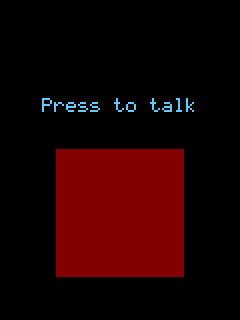
\includegraphics[width=\textwidth]{cap_audio_inact}
		\caption{Released}
		\label{fig:capAudioInAct}
	\end{subfigure}
	\begin{subfigure}[b]{0.4\columnwidth}
		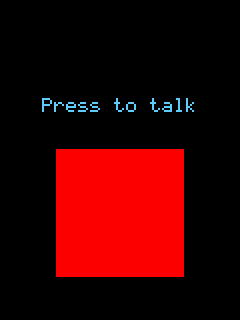
\includegraphics[width=\textwidth]{cap_audio_act}
		\caption{Pressed}
		\label{fig:capAudioAct}
	\end{subfigure}
	\caption{Audio controller GUI}
	\label{fig:capAudio}
\end{figure}
\vspace{6pt}
\else
\begin{figure}[H]
	\centering
	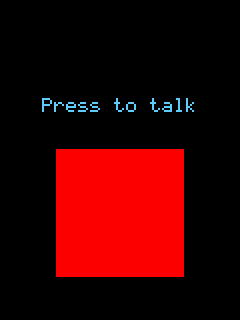
\includegraphics[width=0.4\columnwidth]{cap_audio_act}
	\caption{Audio controller GUI}
	\label{fig:capAudio}
\end{figure}
\vspace{6pt}
\fi

After pressed or released the button, Il Matto 1 send a command to Il Matto 2 to enable or disable audio transmit.
\vspace{6pt}

% Notification system design
\fontSubHeading
\stepcounter{subsections}
\textbf{\thesections.\thesubsections\tab Notification system design}
\vspace{6pt}

Notification system was designed to handle incoming messages and requests. It store the messages and requests by first-in-first-out, than displayed when the user is free, e.g. at menu mode. Example incoming request and text message GUI shown in Figure \ref{fig:capNTC}. Source code listed at 6 and 7 attached with group report.

\begin{figure}[H]
	\centering
	\begin{subfigure}[b]{0.4\columnwidth}
		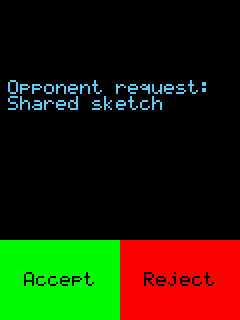
\includegraphics[width=\textwidth]{cap_req}
		\caption{Sketch request}
		\label{fig:capReq}
	\end{subfigure}
	\begin{subfigure}[b]{0.4\columnwidth}
		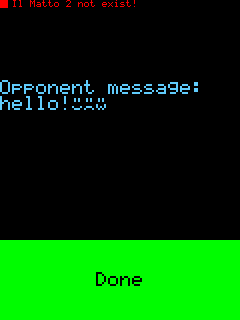
\includegraphics[width=\textwidth]{cap_msg}
		\caption{Text message}
		\label{fig:capMsg}
	\end{subfigure}
	\caption{Notification system GUI}
	\label{fig:capNTC}
\end{figure}
\vspace{6pt}

% UART communcation protocol design
\fontSubHeading
\stepcounter{subsections}
\textbf{\thesections.\thesubsections\tab UART communication protocol design}
\vspace{6pt}

UART0 on the ATmega644P microcontroller was used for communication between Il Matto 1 and Il Matto 2. Interrupts and acknowledge used for lossless data transmit and receive. Double buffer was implemented, so that the communication could be full duplex, and microcontroller could be dealing with one package while the UART interrupts were transmitting another one to improve time slot efficiency. Source code listed at 14 and 15 attached with group report.
\vspace{6pt}

Data was packaged with a maximum size of 64 bytes, detailed as follows:
\vspace{6pt}

\begin{enumerate}[label={\arabic*)},align=left,leftmargin=0.5cm,labelwidth=!,topsep=0pt,partopsep=0pt,parsep=0pt,itemsep=0pt]
\item Command (1 byte), the required operation. Commands without COM\_DATA macro does not have data, length byte would not transmitted as well.
\item Length (1 byte).
\item Data (Maximum 64 bytes).
\end{enumerate}
\vspace{6pt}

The commands were defined in 'communcation.h' header file, listed at 33 attached with group report.
\vspace{6pt}

To help with coding, flow chats were drawn, attached at Appendix \ref{apx:uartTX} and \ref{apx:uartRX}.
\vspace{10pt}

% Testing & Results
\fontHeading
\stepcounter{sections}
\textbf{\thesections.\tab Testing \& Results}
\vspace{10pt}

\fontBody
Since the entire GUI is coded by one person only, the integration of modules for GUI was done at design stage, working together without any problem.
\vspace{6pt}

% Menu selection GUI
\fontSubHeading
\stepcounter{subsections}
\textbf{\thesections.\thesubsections\tab Menu selection GUI}
\vspace{6pt}

\fontBody
The menu selection GUI involves a complex coordinate translate and drawing algorithm, was the most buggy part, but all solved. It was tested by some different ways, scroll quickly tests for large area refresh, scroll slowly tests for small area refresh at the edge and changing top and bottom fixed area tests coordinate transform. All of them worked as expected.
\vspace{6pt}

% Touchscreen
\fontSubHeading
\stepcounter{subsections}
\textbf{\thesections.\thesubsections\tab Touchscreen}
\vspace{6pt}

\fontBody
Originally landscape orientation was chosen, after implemented some code for read and calibrate touchscreen \ref{ref:librTouch}, the touchscreen was tested by plotting points onto TFT, however the points plotted were very noisy as shown by photo \ref{fig:photoTSNoisy}.
\vspace{6pt}

\begin{figure}[H]
	\centering
	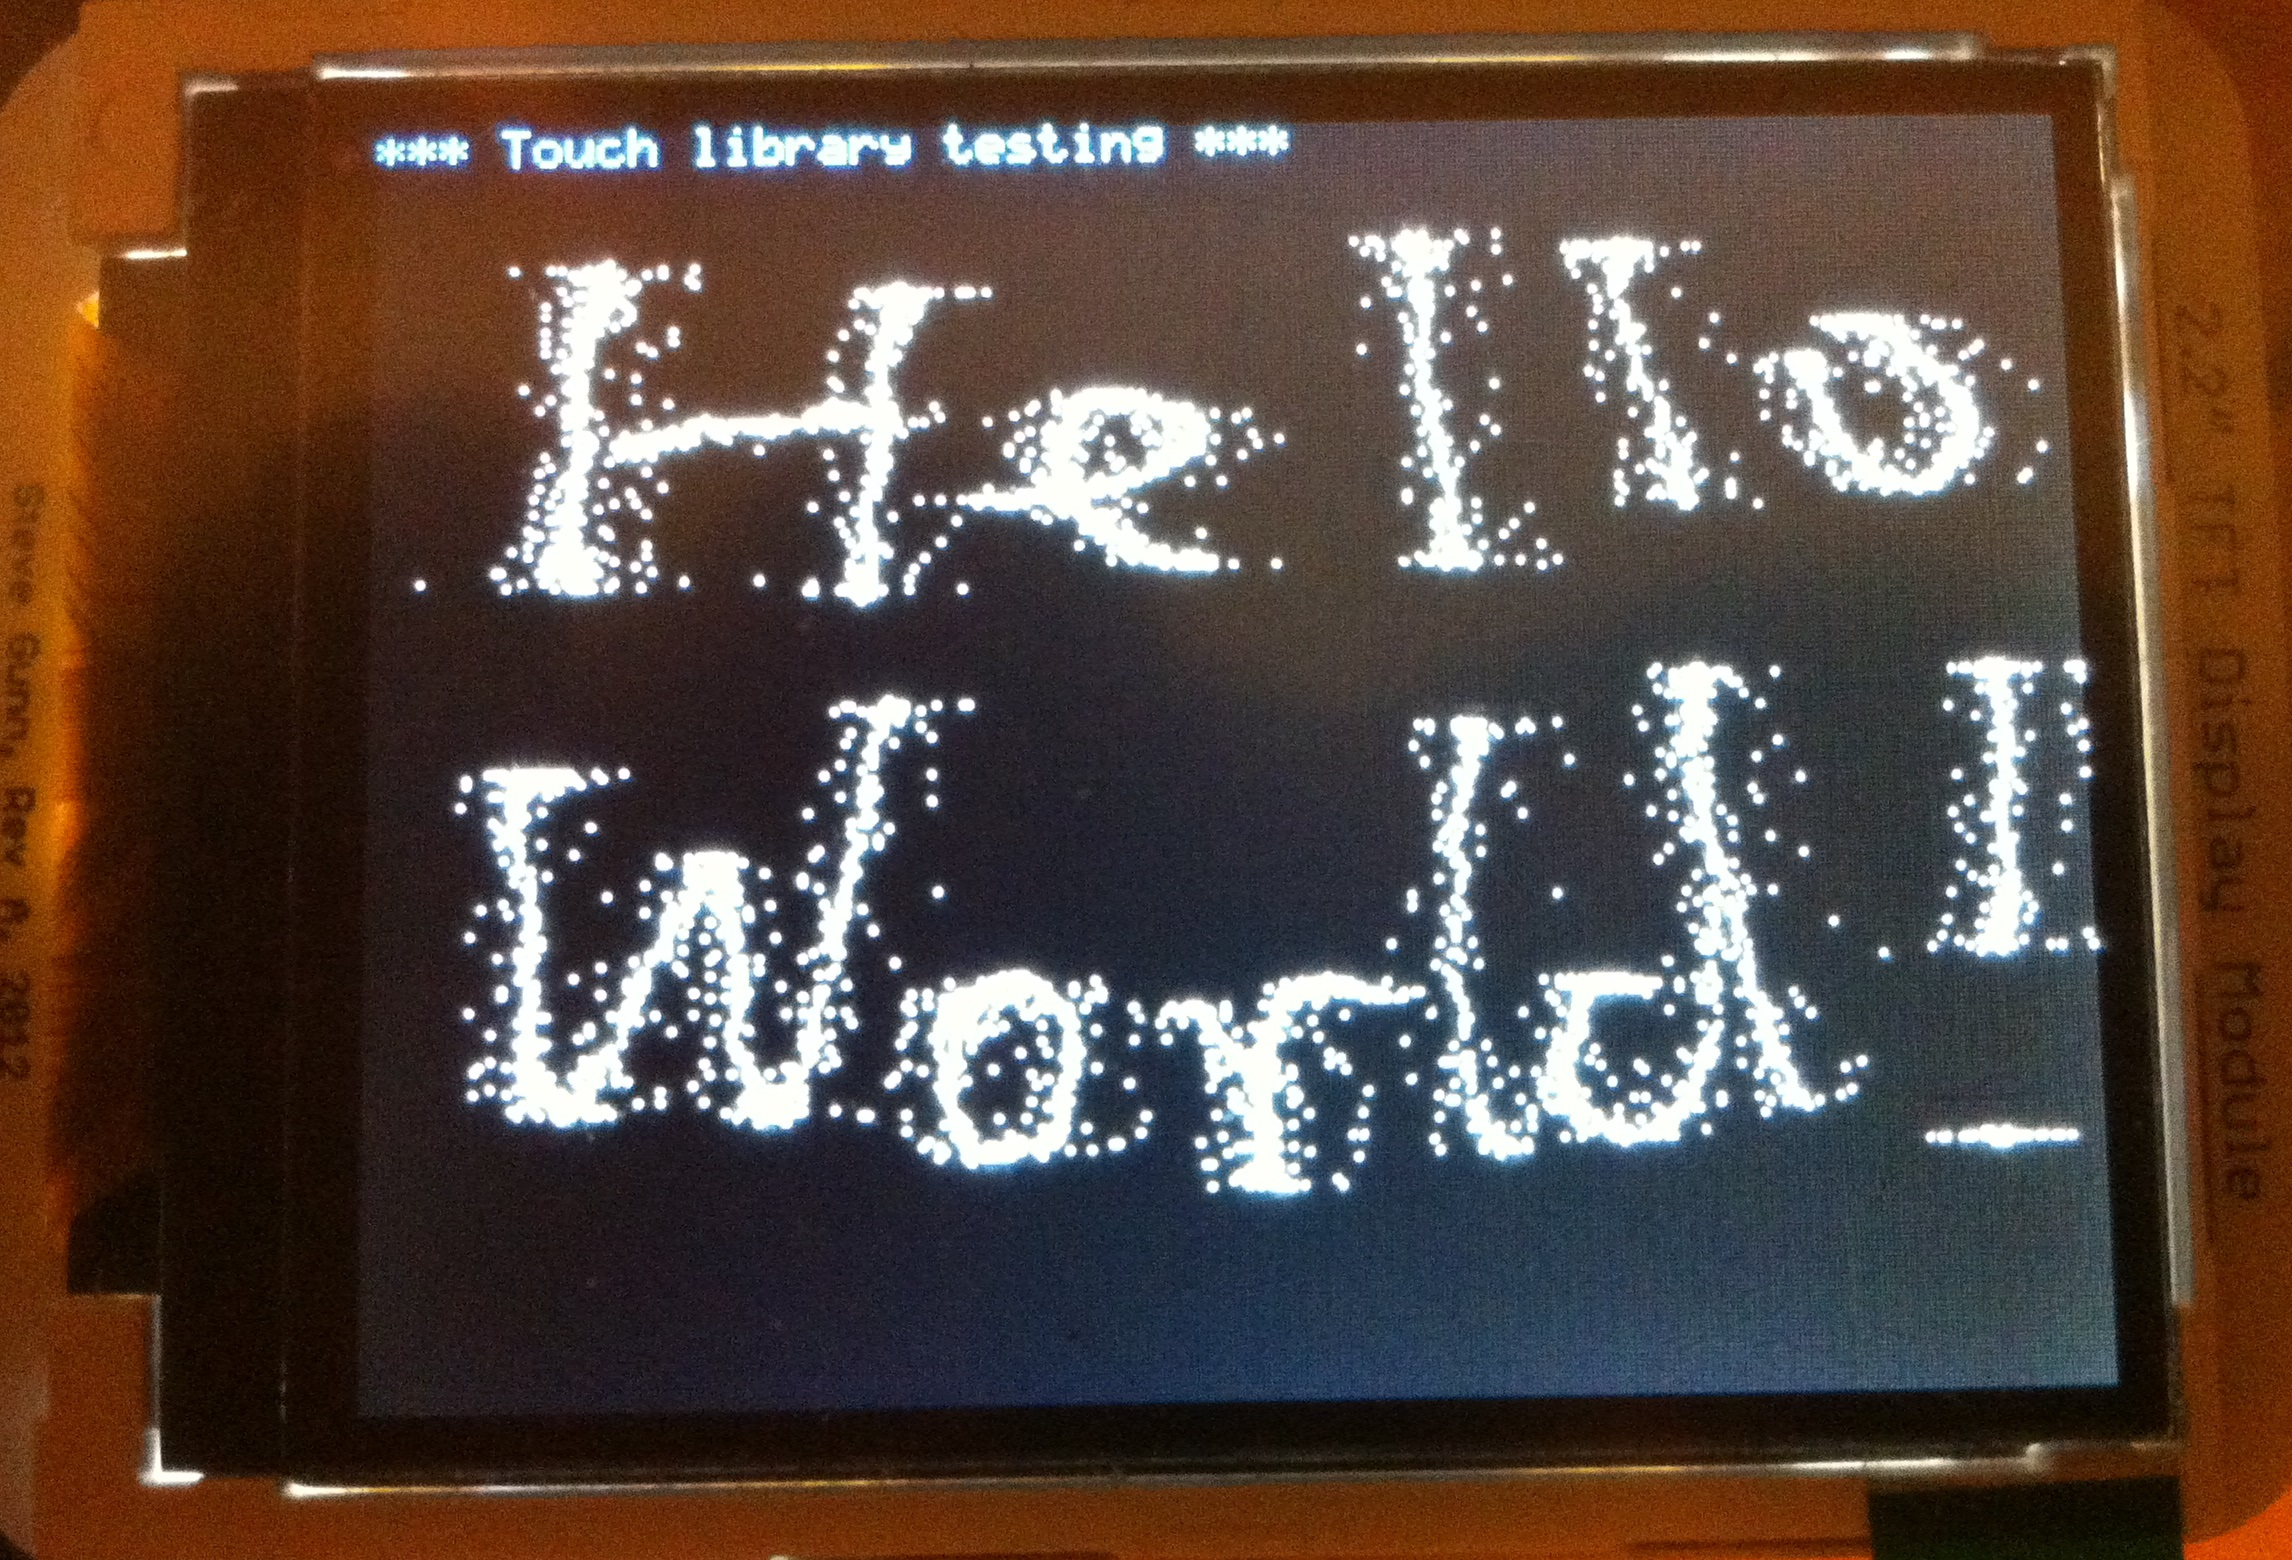
\includegraphics[width=0.6\columnwidth]{photo_ts_noisy}
	\caption{Touchscreen noisy when placed on top of TFT}
	\label{fig:photoTSNoisy}
\end{figure}
\vspace{6pt}

The touchscreen noise reduced dramatically while holding up, therefore the final orientation of the device decided to be portrait, using the box for Il Matto to support it underneath the edge, which would gave some space between the touchscreen and TFT. Later changed to a 3D printed case designed by dh1g14.
\vspace{6pt}

For reduce touchscreen noises further, a software ADC averager was implemented with glitch filter \ref{ref:librTouch}, result demonstrated by Figure \ref{fig:capTSAvg}.
\vspace{6pt}

\begin{figure}[H]
	\centering
	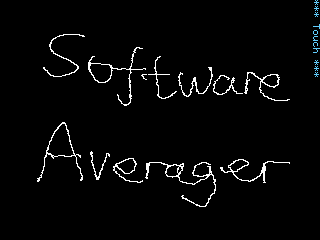
\includegraphics[width=0.6\columnwidth]{cap_ts_avg}
	\caption{Touchscreen sketch after software averager}
	\label{fig:capTSAvg}
\end{figure}
\vspace{6pt}

Near the end of prototyping, one of the touchscreen was damaged, produces glitches and panning in x direction, made sketch not understandable, causing difficulty in keypad input and pressing menu items. The other touchscreen has the same problem as well, but not as severe as the former one. This was probably because of inappropriate assembly and frequent removing of the touchscreen without enough care. The two thin resistive layer on top of the touchscreen split by a small space, twist of the touchscreen during removing would easily cause the top layer to distort, damage the entire touchscreen.
\vspace{6pt}

% Communcation
\fontSubHeading
\stepcounter{subsections}
\textbf{\thesections.\thesubsections\tab Communication}
\vspace{6pt}

The UART communication protocol designed was the same for transmitter and receiver, thus could be easily tested by using two Il Matto 1 connected together, after implemented some basic commands like ping. A submenu with diagnosis function also implemented, mainly for testing UART communication, as shown in Figure \ref{fig:capDiag}. One Il Matto could be configured to pooling for data, another one send different data packages from shared sketch mode etc. to test data packaging functionality, or try to send lots of data to test for data loss.

\begin{figure}[H]
	\centering
	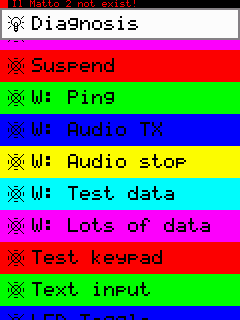
\includegraphics[width=0.4\columnwidth]{cap_diagnosis}
	\caption{Diagnosis menu}
	\label{fig:capDiag}
\end{figure}
\vspace{6pt}

During test, some critical bugs found. The initial version wrote without utilise flow chart could not do full duplex, therefore the entire UART module almost rewrote. Another bug found was both end might waiting for acknowledge at the same time, completely blocked UART communication, was corrected in current version.
\vspace{6pt}

Current version of UART communication module worked without any problem. Double buffer, wait for acknowledge before send the next package all worked as expected. Also tested by connect two Il Matto 1, than using shared sketch mode, sketch at both side very quick at the same time, which would produce lots of data packages at both end quickly. None of either side ever stopped responding or lost a portion of sketch, indicates the UART module worked as expected.
\vspace{6pt}

% Integration
\fontSubHeading
\stepcounter{subsections}
\textbf{\thesections.\thesubsections\tab Integration}
\vspace{6pt}

\fontBody
The interface designed for UART module made integration with Il Matto 2 fairly easy. After implemented some essential commands like ping, send and receive data packages on Il Matto 2 within hours, both end communicated through wireless successfully. At short distance, sketch transmitted to either side instantly, but might lost when trying to sketch on both side at the same time, because the wireless module could not do full duplex transmission. At greater distance, sketch data start to loss. That was approximately 5 meters in the computer lab, improved a lot outside the computer lab. That could also be improved after implemented data acknowledge at Il Matto 2, which was not implemented because of time constrains.
\vspace{6pt}

The audio controller press-to-talk button worked as expected after implemented audio start and audio stop commands on Il Matto 2.
\vspace{6pt}

Text messages could be sent to either side without data loss or corruption, mainly because the data packages will be automatically resent if acknowledge not received within a period of time implemented on Il Matto 1.
\vspace{6pt}

Because of the acknowledge functionality of UART communication, if Il Matto 2 stopped responding, Il Matto 1 could also stuck. Generally the indicator on top left of Il Matto 1 TFT would turn to red indicates Il Matto 2 stopped responding. In this case, reset the whole system would bring them back to working state.
\vspace{10pt}

% Team Working
\fontHeading
\stepcounter{sections}
\textbf{\thesections.\tab Team Working}
\vspace{10pt}

\fontBody
The ideas of the device was collected firstly, so that everyone could choose what they were good at. That become more detailed after we got the block diagram of the device. Since we were 6 students, every 2 were assigned to a particular task. I were assigned to Il Matto 1 GUI design and UART communication with Diwen (dh1g14), while Alaa and Nathan assigned to analog stuff including microphone amplifier and loudspeaker amplifier, Joseph and Fiona were going to get wireless transmission module working.
\vspace{6pt}

Facebook group created at our first meeting, so in case anyone has any ideas or questions we can discuss it online. For example, when I found out landscape orientation was not working, I got some ideas from Facebook instantly.
\vspace{6pt}

Source code were shared and managed through SourceKettle. But only I and Nathan were using it, because of the complicated things to learn at first time.
\vspace{6pt}

The team were managed 'flatly', everyone were able to help others. Targets were requested by everyone from where they were good at to be most productive. Team leader was mainly care about progress, time and meeting arrangement.
\vspace{6pt}

Risks were planned as in Risk Management table. The only unexpected event would be the damage of touchscreen, but we could not do anything about it actually, we did not have enough budget to buy another touchscreen, the damaged touchscreen was actually still useable but just not stable.
\vspace{10pt}

% Reflection
\fontHeading
\stepcounter{sections}
\textbf{\thesections.\tab Reflection}
\vspace{10pt}

\fontBody
We planned SD card, data acknowledge through wireless communication and some other ideas, but had not got time to implement them. Text message implemented on the last day, without intensive test and debug.
\vspace{10pt}

\iffalse
% ****************************************** COMMENTS ******************************************
\begin{gather}
	I_c = \beta I_b
	\label{eq:cc_ic}\\
	I_{R_{3,4}} \gg I_{b2}
	\label{eq:cc_ir34}
\end{gather}
\parskip=6pt

\begin{equation}
	I_e = I_c + I_b = \left( 1 + \beta \right) I_b
	\label{eq:cc_ie}
\end{equation}
\parskip=6pt
% ****************************************** COMMENTS ******************************************
\fi

\fontHeading
\textbf{References}
\vspace{10pt}

\fontRef
\begin{enumerate}[label={[\arabic*]},align=left,leftmargin=0.7cm,labelwidth=!,topsep=0pt,partopsep=0pt,parsep=0pt,itemsep=0pt]
\item
\label{ref:ili9341}
ILITEK "ILI9341 specification" [\textit{Online}]. Available: \url{https://www.adafruit.com/datasheets/ILI9341.pdf}
\item
\label{ref:tsATMEL}
ATMEL "AVR341: Four and five-wire Touch Screen Controller" [\textit{Online}]. Available: \url{http://www.atmel.com/images/doc8091.pdf}
\item
\label{ref:tsNXP}
NXP "Interfacing 4-wire and 5-wire resistive touchscreens to the LPC247x" [\textit{Online}]. Available: \url{http://www.nxp.com/documents/application_note/AN10675.pdf}
\item
\label{ref:tsTI}
Texas Instruments "Calibration in touch-screen systems" [\textit{Online}]. Available: \url{http://www.ti.com/lit/an/slyt277/slyt277.pdf}
\item
\label{ref:tslib}
K. Russell, L. Douglas, L. Chris "tslib-1.0" [\textit{Online}]. Available: \url{https://packages.debian.org/source/wheezy/tslib}
\item
\label{ref:libtft-cpp}
Z. Yubo (yz39g13) "libtft-cpp" [\textit{Online}]. Available: \url{https://github.com/zhiyb/Il-Matto/tree/master/lib/libtft-cpp}
\item
\label{ref:librTouch}
Z. Yubo (yz39g13) "librTouch" [\textit{Online}]. Available: \url{https://github.com/zhiyb/Il-Matto/tree/master/lib/librTouch}
\item
\label{ref:liblist}
Z. Yubo (yz39g13) "liblist" [\textit{Online}]. Available: \url{https://github.com/zhiyb/Il-Matto/tree/master/lib/liblist}
\end{enumerate}

\end{multicols}

% Appendix. UART TX flow chat
\newpage
\fontHeading
{\refstepcounter{appendix}\label{apx:uartTX}}
\textbf{Appendix \theappendix:\tab UART transmit flow chat}
\vspace{10pt}

\begin{figure}[H]
	\centering
	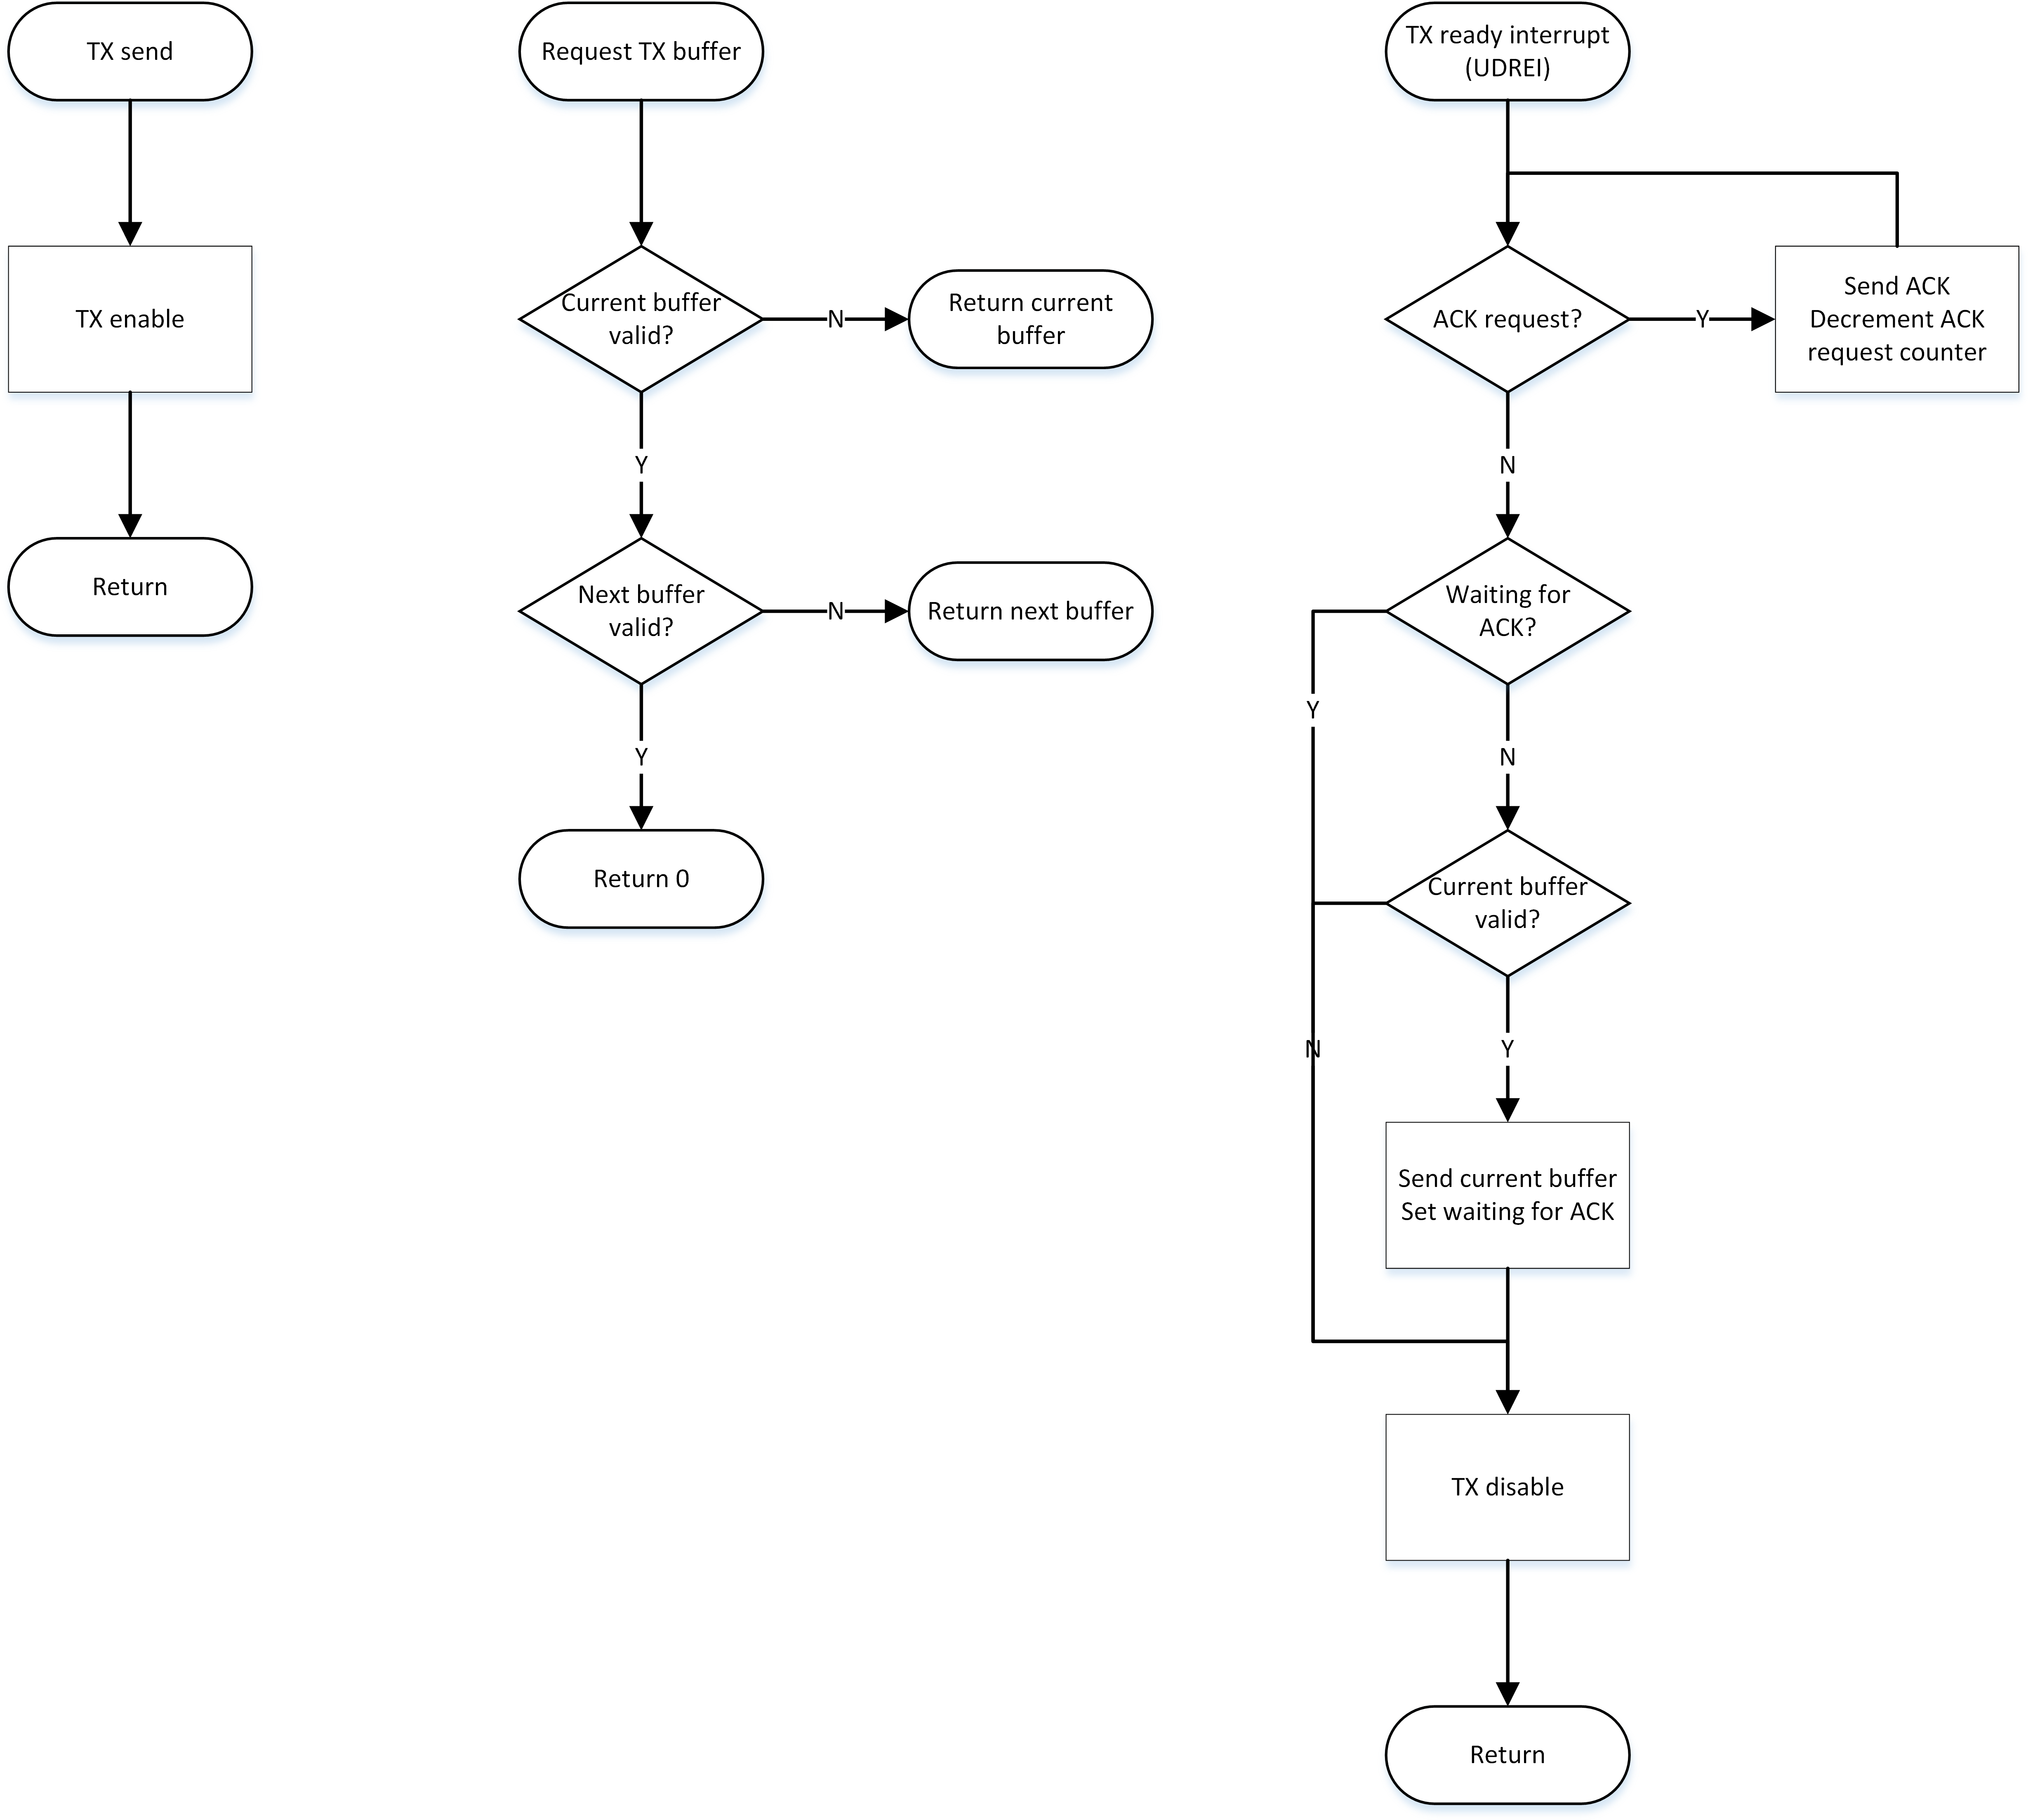
\includegraphics[width=\columnwidth]{uart_tx}
\end{figure}

% Appendix. UART RX flow chat
\newpage
\fontHeading
{\refstepcounter{appendix}\label{apx:uartRX}}
\textbf{Appendix \theappendix:\tab UART receive flow chat}
\vspace{10pt}

\begin{figure}[H]
	\centering
	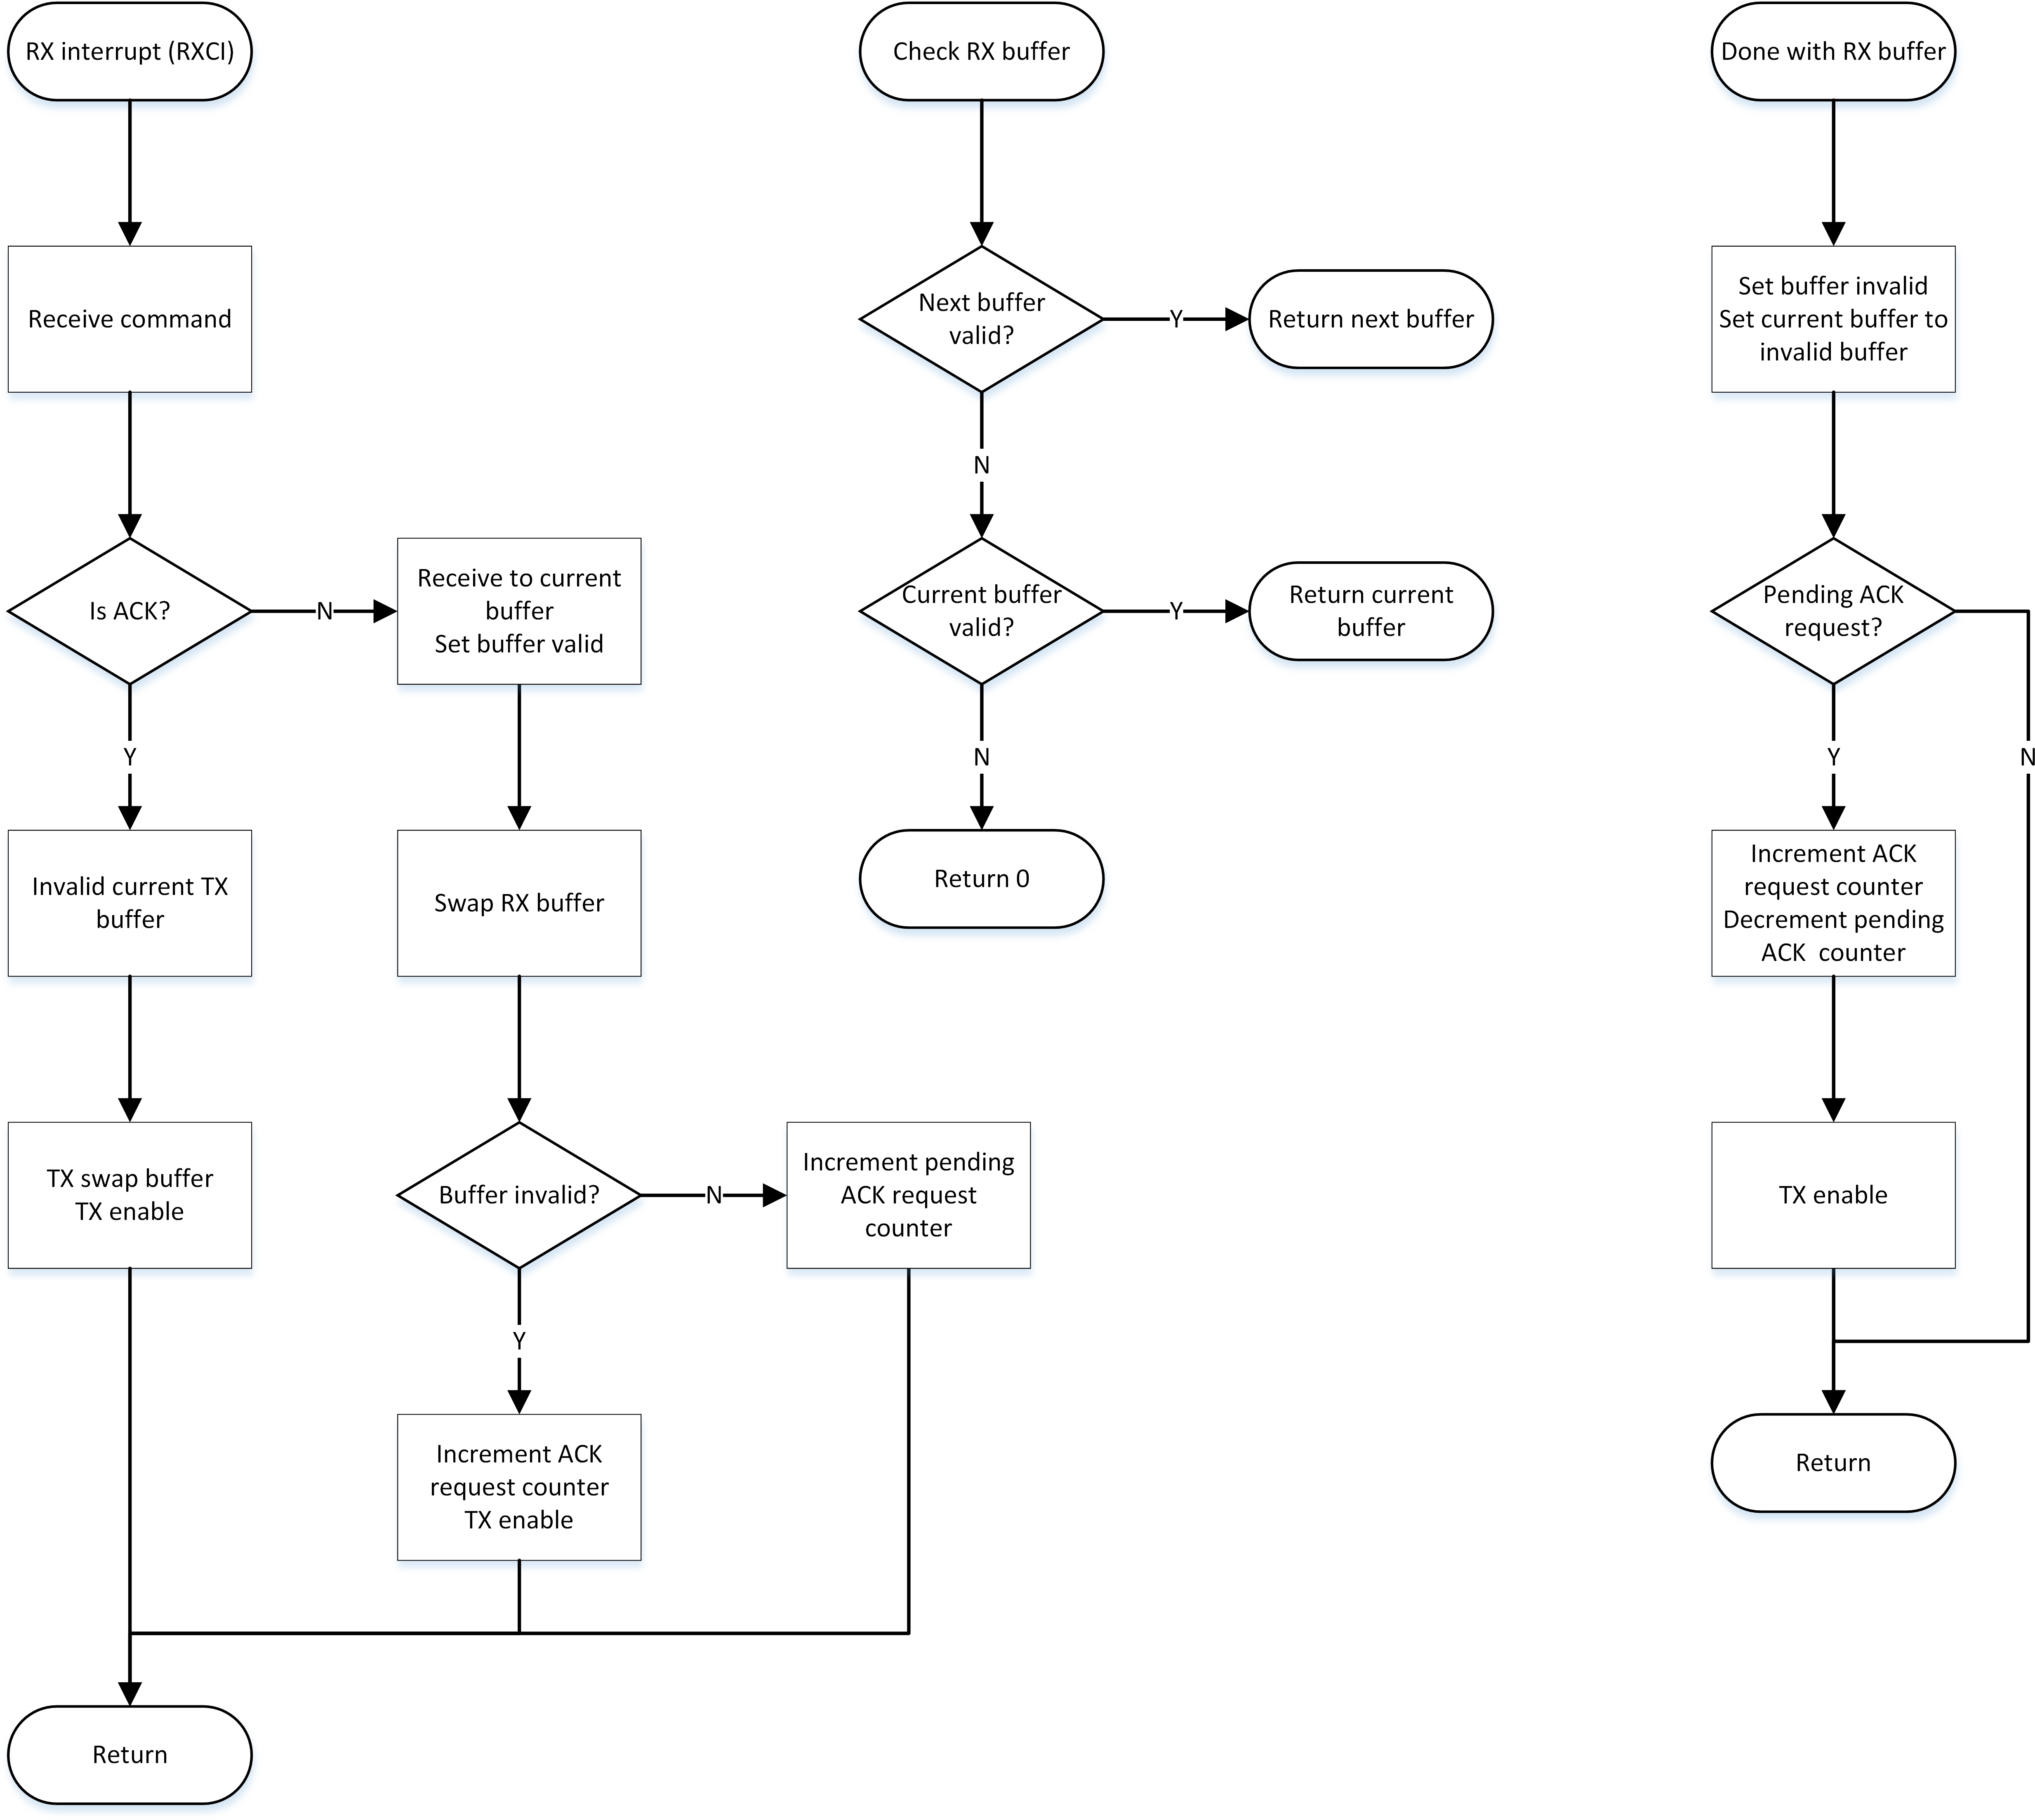
\includegraphics[width=\columnwidth]{uart_rx}
\end{figure}

\end{document}
